\subsection{Architektúra}

A szoftver egészében és komponenseiben is rétzegzett architektúrát valósít meg, melynek egy áttekintő ábrája látható a \ref{fig:architecture} ábrán.

\begin{figure}[H]
    \centering
    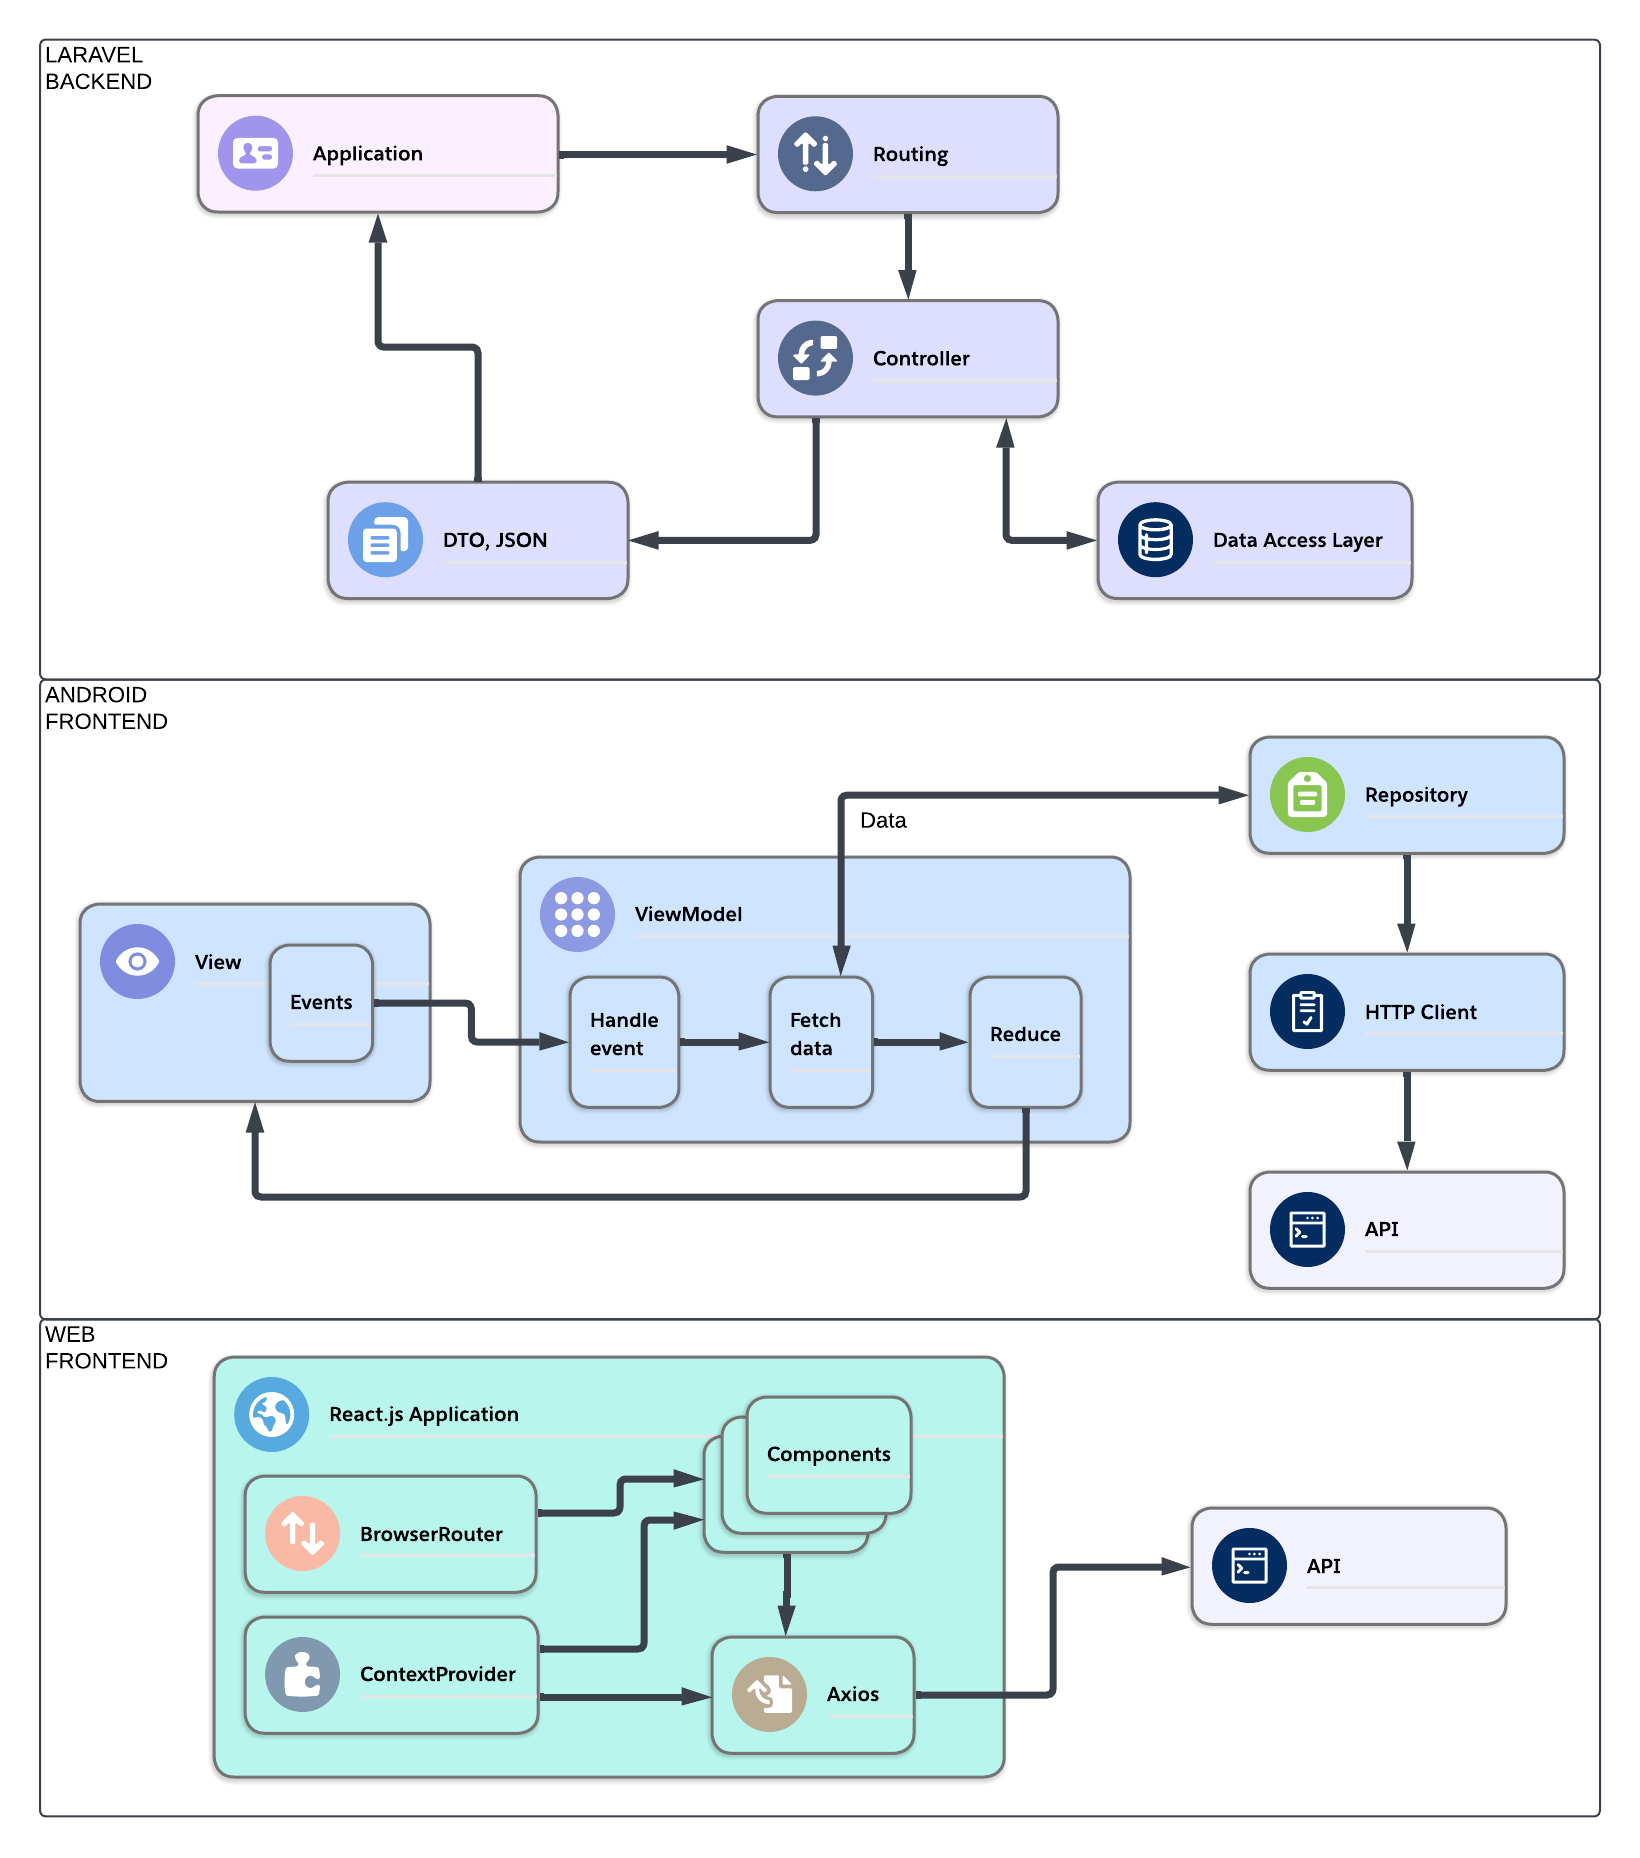
\includegraphics[scale=0.5]{./figures/architecture.png}
    \caption{A szoftver architektúrája}
    \label{fig:architecture}
\end{figure}

A szoftver egy kliens-szerver architektúrát valósít meg, ahol a kliensek a szerverrel REST API-n keresztül kommunikálnak. A szerver oldali alkalmazás a Laravel PHP keretrendszer segítségével készült, míg a kliens oldali alkalmazás két részre osztható: egy webes frontendre, mely a React keretrendszerre épül, és egy mobil kliensre, mely a JetPack Compose keretrendszer segítségével készült.

\subsubsection{Backend architektúra}

A Laravel alapból az MVC (Model-View-Controller) architektúrát követi, azonban a projektünkben a nézeteket a kliensek kezelik, így csak a Modell és a Controller rétegek maradnak meg. Így a Laravel alkalmazásunk 2 fő rétegre osztható:

\begin{itemize}
    \item Adathozzáférési réteg (Data Access Layer)
    \item Üzleti logikai réteg (Business Logic Layer)
\end{itemize}

A kliensekkel való kommunikáció REST API-n keresztül történik, így a Laravel alkalmazásunkban a REST API végpontok implementációja a kontrollerekben található. A küldött és fogadott adatok JSON formátumban vannak, melyek a Laravel által biztosított Resource osztályok segítségével könnyen kezelhetőek, melyek egyfajta DTO (Data Transfer Object) mintaként működnek.

\subsubsection{Mobilos kliens}

A mobilos kliens 2 fő rétegre osztható:

\begin{itemize}
    \item  [1.] Adat réteg (Data Layer)
    \begin{itemize}
        \item Adatlekérdezési réteg (HTTP kliens): REST API hívások implementációja, JSON objektumok kotlin osztályokra való leképezése.
        \item Adatelérési réteg (Repository): hálózati kommunikáció és hibakezelés és egységesített kezelése, magasabb szintű kódban könnyebben használható.
    \end{itemize}
    \item  [2.] UI réteg (UI Layer)
    \begin{itemize}
        \item  Állapotkezelés (View Model)
        \item  Megjelenítés (View)

    \end{itemize}
\end{itemize}